\subsection{External Communication}
\label{design:communication}

Since we will use a 2-tiered approach for the bootware component, we now have to decide, how the communication between the two components will work.
There are several factors that impact this decision.

Communication between the components should be as simple as possible, but has to support some critical features.

Since the provisioning processes kicked off by the bootware can potentially take a lot of time to finish (in the range of minutes to hours), asynchronous communication should be used between the components to avoid timeouts and blocking resources.

For the same reason, there should be some mechanism to get feedback on the current status during a long running provisioning process.

There will be other components that have to call the bootware to start some provisioning process, so communication has to be open for other parties.

The communication with the bootware components will contain sensitive data, for example login information for cloud providers that the bootware needs to do its job, but has to be provided from the outside on a call to call basis.
This information has to be transported securely to prevent malicious or fraudulent attacks.
The selected communication method therefore has to support some sort of security mechanisms, ideally end-to-end security via message encryption.
While these security mechanisms will not be used in this thesis due to time constraints, selecting the right communication method is still critical for future development.

Since this whole project is concerned with services, it \textcolor{red}{liegt nahe} to use web service calls and returns as main communication method, internally as well as  externally.
This way we offer a consistent interface for all components to use.
\autoref{image:webservice} shows the addition of asynchronous web service call and return communication to the proposed architecture.
Using a web service with soap messaging also gives us access to Web Service Security Framework, which supports end-to-end security with encryption and signatures.

\begin{figure}[!htbp]
	\centering
	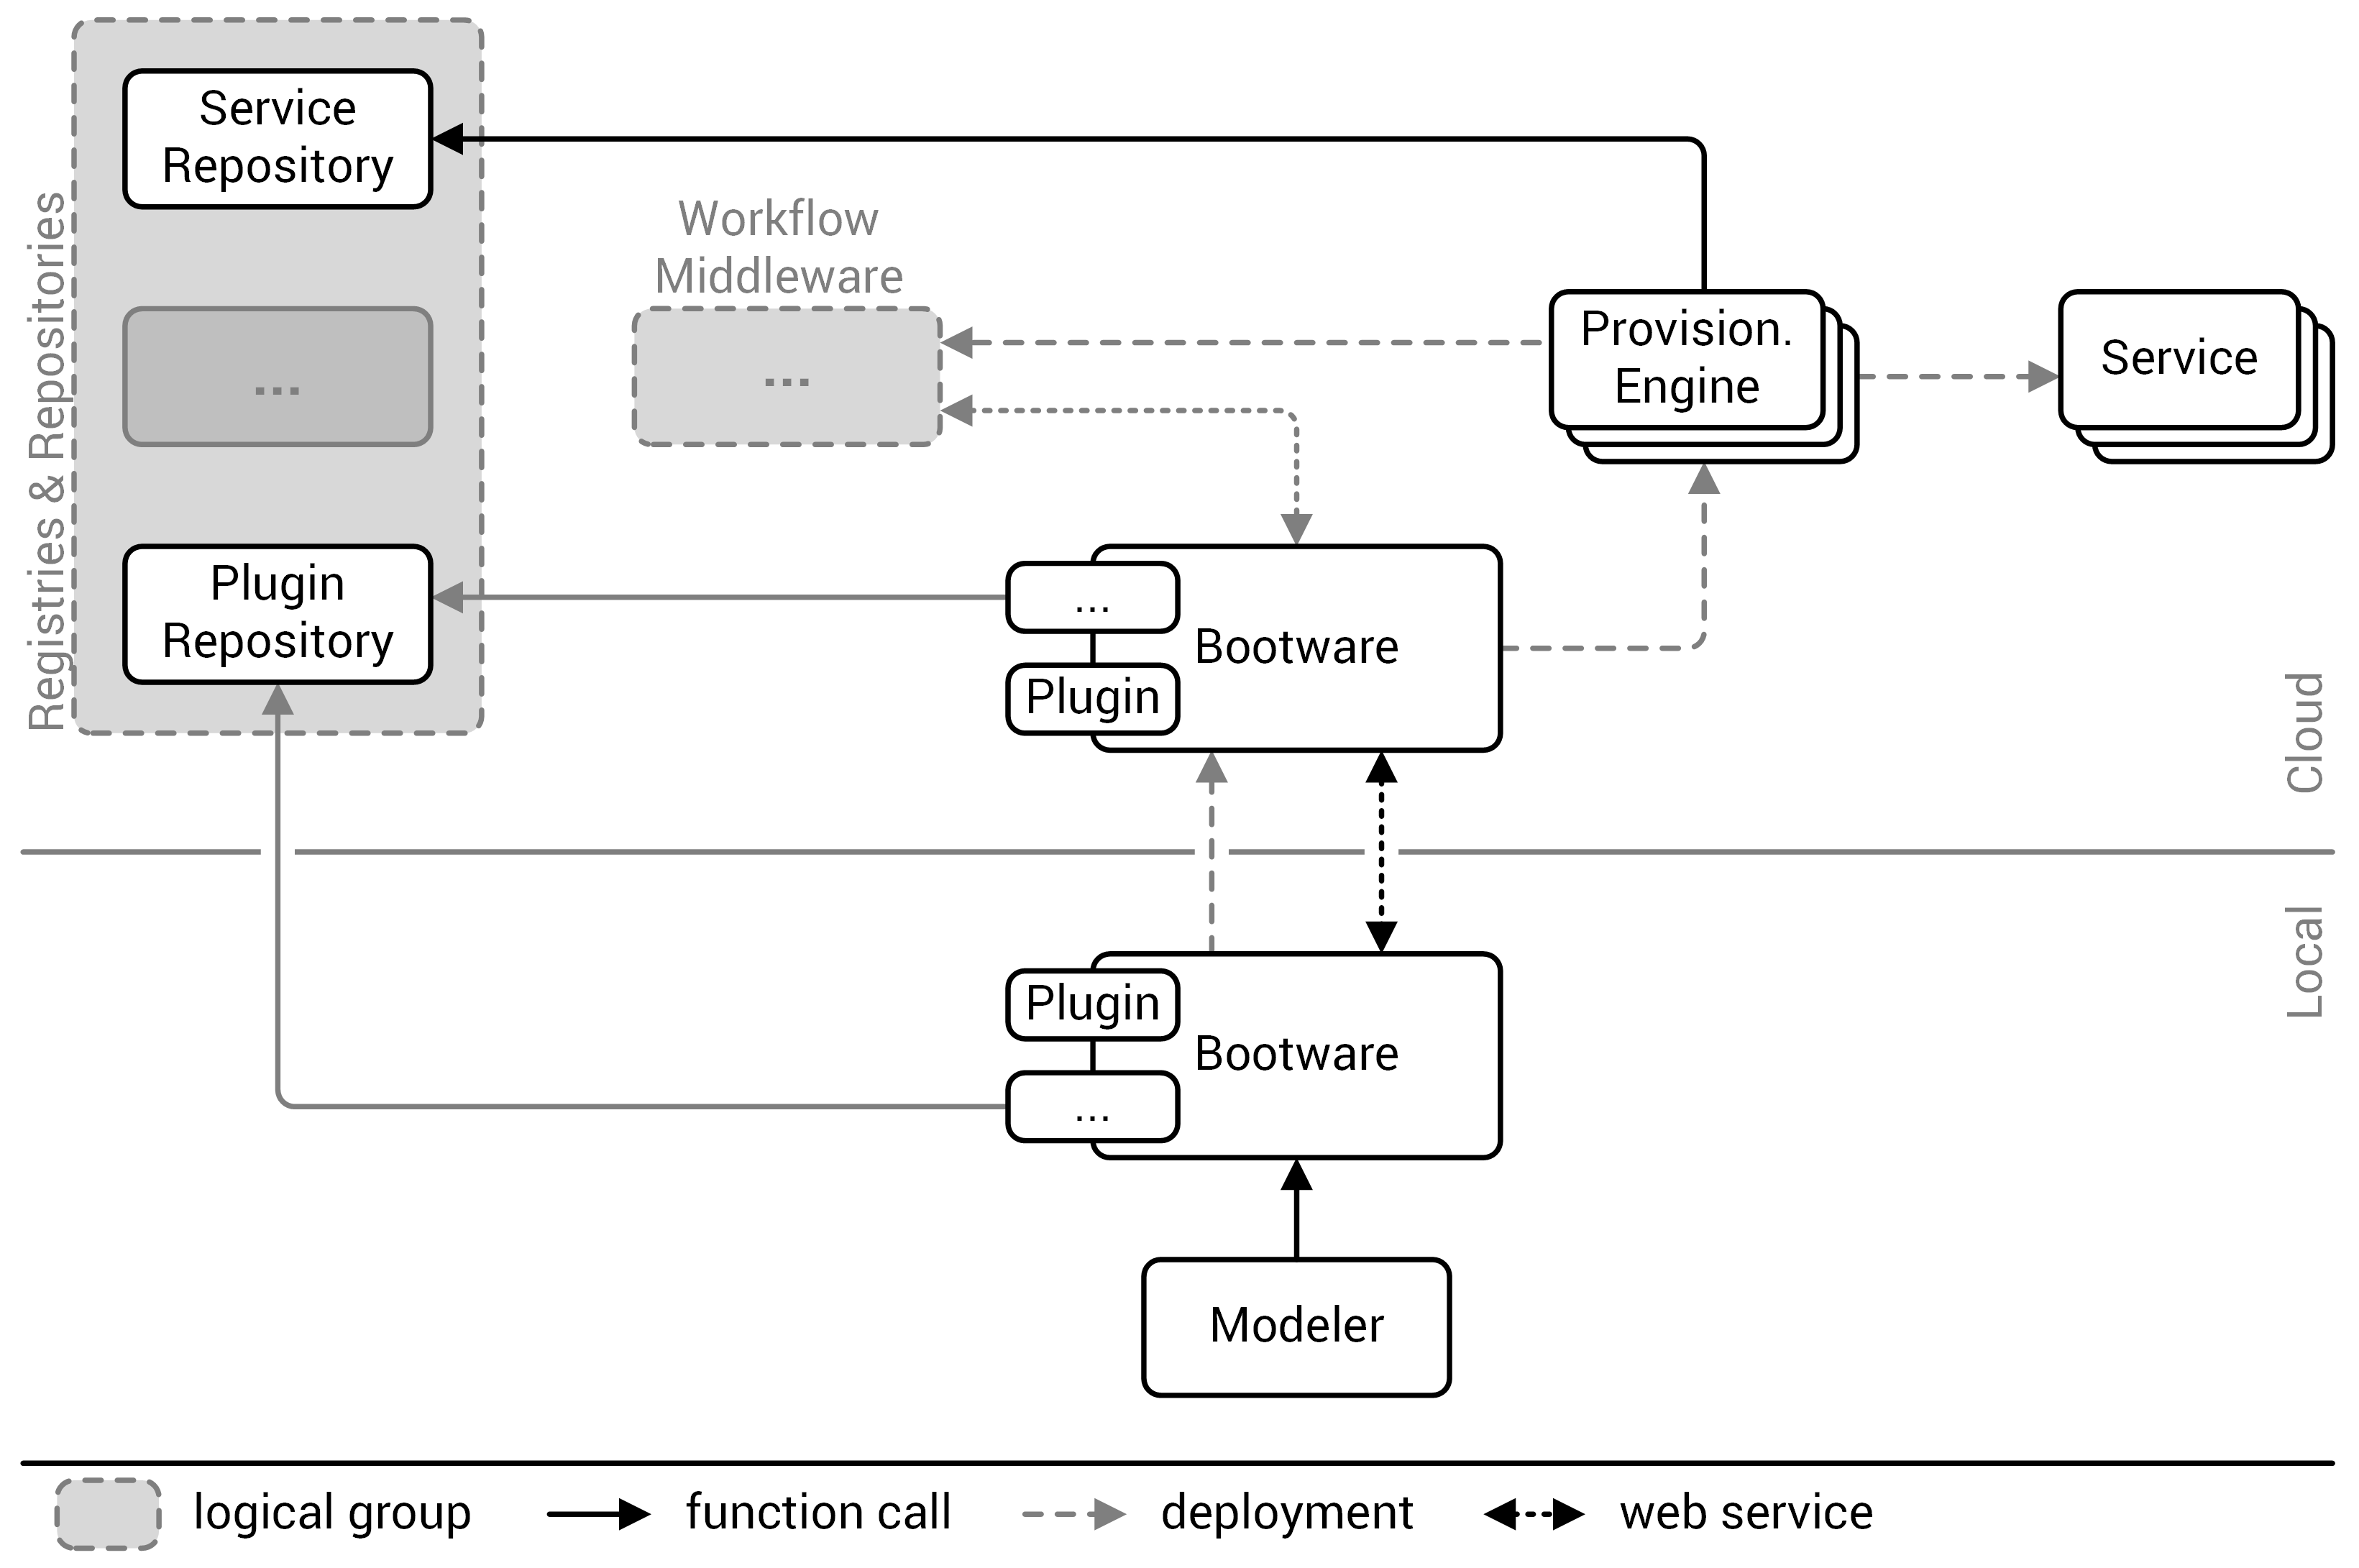
\includegraphics[resolution=600]{design/assets/simple_webservice}
	\caption{Simplified overview of the 2-tier architecture with asynchronous web service communication}
	\label{image:webservice}
\end{figure}

Web Services also support asynchronous communication so that long running provisioning processes won't pose a problem.
We do however still need information during those long running processes to give the user some feedback.
This can't (\textcolor{red}{???}) be accomplished by this simple request/response pattern.
For this, a secondary communication mechanism which supports sending multiple feedback messages has to be used.

Since it is not necessary for the successful use of the bootware it would make sense to implement this secondary communication mechanism as a plugin.
This would allow us to add arbitrary communication plugins to the bootware depending on future needs.

One natural choice for this is the PubSub pattern implemented by some messaging middleware.
Using this pattern, the remote bootware component pushes messages to a message queue to which the local bootware component (and other components if needs be) can subscribe to receive future messages.
\autoref{image:queue} shows an additional message queue.

\begin{figure}[!htbp]
	\centering
	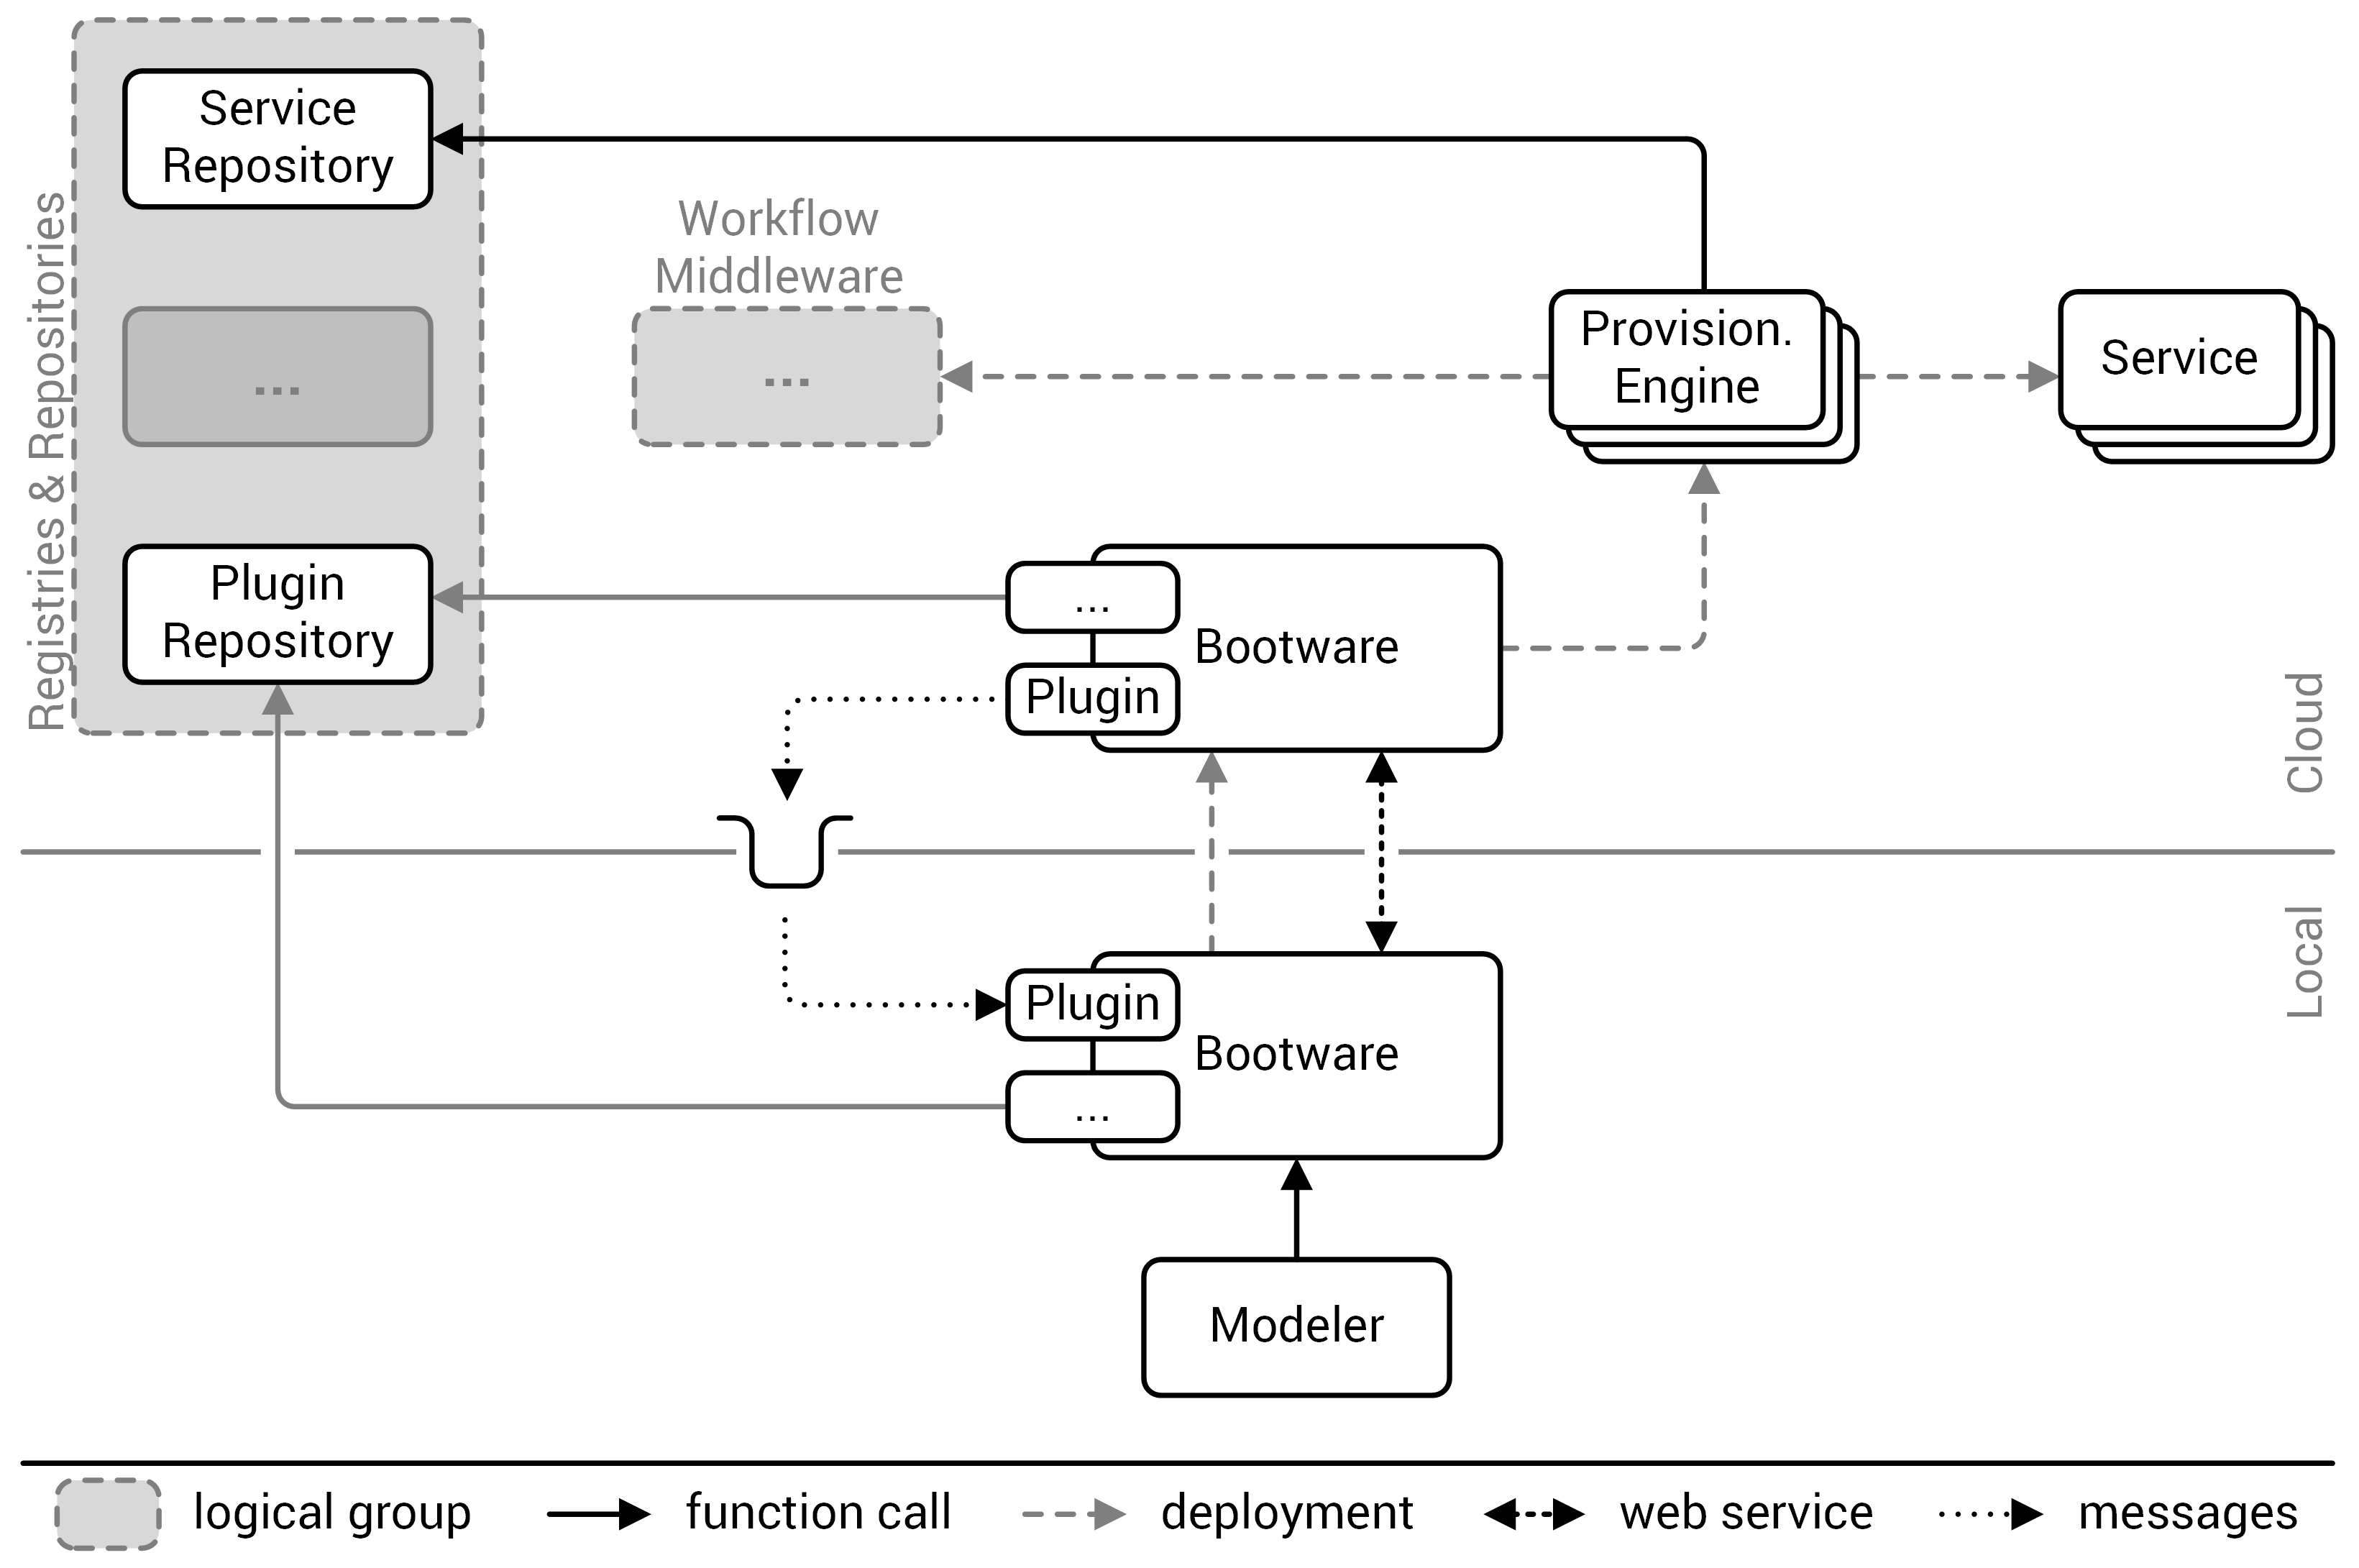
\includegraphics[resolution=600]{design/assets/simple_queue}
	\caption{Simplified overview of the 2-tier architecture with asynchronous web service and a messaging queue communication}
	\label{image:queue}
\end{figure}
